\documentclass[a4paper,10pt]{book}
\usepackage[english]{babel}     
\usepackage[utf8]{inputenc}     % accent symbols
\usepackage[T1]{fontenc}
\usepackage{lmodern}
\usepackage{microtype}
\usepackage{natbib}
\usepackage{tocbibind}          
\usepackage{amsmath}            % math symbols
\usepackage{amsthm}             % math symbols
\usepackage[colorlinks=true,linkcolor=red]{hyperref} % hyper link

% for code
\usepackage{listings}
\usepackage{color,xcolor}
\definecolor{mygreen}{rgb}{0,0.6,0}
\definecolor{mygray}{rgb}{0.9,0.9,0.9}
\definecolor{mymauve}{rgb}{0.58,0,0.82}
\lstset{
backgroundcolor=\color{mygray},
numbers=left,                    
columns=fullflexible,
breaklines=true,      
captionpos=b,         
tabsize=4,            
commentstyle=\color{mygreen}, 
escapeinside={\%*}{*)},       
keywordstyle=\color{blue},    
% stringstyle=\color{mymauve}\monaco,
frame=single,                        
rulesepcolor=\color{red!20!green!20!blue!20},
% identifierstyle=\color{red},
%% language=c++,
basicstyle=\tiny
}

\usepackage{indentfirst}
\setlength{\parindent}{2em}
\usepackage[onehalfspacing]{setspace}
% graph
\usepackage{pdfpages}
\usepackage{graphicx}
% box
\usepackage{booktabs}
\usepackage{tcolorbox}

%% user defined command
\newcommand{\keyword}[1]{\textbf{#1}}
\newcommand{\keywords}[1]{\textbf{#1}}
\newcommand{\lcmd}[1]{\texttt{#1}}
\newcommand{\head}[1]{\textnormal{\textbf{#1}}}
\newcommand{\itwords}[1]{\textit{#1}}

\usepackage{float}
% all symbols
\usepackage{tipa}
\usepackage{tipx}

\usepackage{datetime}
% \usepackage{movie15}


% variable
% TODO
\newcommand{\pdfauthor}{李明明}
\newcommand{\pdftitle}{工作}
\newcommand{\pdfsubject}{工作中的经验与教训}
\newcommand{\pdfkeywords}{工作经验与教训}
\newcommand{\bookname}{工作收获}
\newcommand{\bookoneword}{工作中吸取的经验和教训}
\newcommand{\timeandcompany}{2020年12月1日}

\usepackage{bm}
\usepackage{amsfonts}
\begin{document}


% Pages are numbered with lowercase Roman numbers.
% Chapters generate a table of contents entry but don't get a number.
\frontmatter{}
\newcommand{\mytitle}{Git}
\newcommand{\firstcreated}{Mar 16, 2023}

\begin{titlepage}

\newcommand{\HRule}{\rule{\linewidth}{0.5mm}} % Defines a new command for the horizontal lines, change thickness here

\center                         % Center everything on the page
 
%----------------------------------------------------------------------------------------
%	HEADING SECTIONS
%----------------------------------------------------------------------------------------


\includegraphics[width=0.5\textwidth]{logo}\\[1cm] % Include a department/university logo - this will require the graphicx package

%----------------------------------------------------------------------------------------
%	TITLE SECTION
%----------------------------------------------------------------------------------------

\HRule\\[0.4cm]
{ \huge \bfseries \mytitle}\\[0.4cm] % Title of your document
\HRule\\[1.5cm]
 
%----------------------------------------------------------------------------------------
%	AUTHOR SECTION
%----------------------------------------------------------------------------------------

\begin{minipage}{0.4\textwidth}
\begin{center} \large
Mingming \textsc{Li}\\ % Your name
\end{center}

\end{minipage}\\[2cm]


%----------------------------------------------------------------------------------------
%	DATE SECTION
% ----------------------------------------------------------------------------------------
\vfill
{\large First Created: \firstcreated}\\
{\large Last Modified: \today}\\[2cm] % Date, change the \today to a set date if you want to be precise



\end{titlepage}


%%% Local Variables:
%%% mode: latex
%%% Tex-master: "git"
%%% End:
\cleardoublepage{}
\phantomsection{}
\tableofcontents{}
\cleardoublepage{}
\phantomsection{}
\listoffigures{}
\cleardoublepage{}
\phantomsection{}
\listoftables{}


% Pages are numbered with Arabic numbers.
% Chapters are numbered and produce a table of contents entry.
\mainmatter{}

\part{Theory}
\label{part:theory}


\chapter{Algorithm}


\section{What is Algorithm?}
\label{sec:what-algorithm}

The following relation show what is an algorithm.
\begin{tcolorbox}
input -> \keyword{algorithm} -> output  
\end{tcolorbox}


An algorithm is a sequence of computational steps that transform the input into the output.
An algorithm describes a specific computational procedure for achieving the input/output relationship.

\section{Instance of a Problem}
\label{sec:instance-problem}


An instance of a problem is the input needed to compute a solution to the problem.

\section{Correct Algorithms}
\label{sec:correct-algorithms}


For every input instance, the algorithm halts out the correct output.
We say the algorithm is correct.


\section[Two Characteristics]{Two Characteristics of Many Algorithms}
\label{sec:two-char-many}

\begin{itemize}
\item There are many candidate solutions, but finding the one that solve or the one is best is challenge.
\item They have practical applications.
\end{itemize}

\section{Data Structure}
\label{sec:data-structure}


Data structure is a way to store and organize data in order to facilitate access and modifications.
No single data structure works well for all purposes, and it is important to know the strengths and limitations of several of them.

\section{The Core Technique}
\label{sec:core-technique}


learn the technique of algorithm design and analysis.

\section{Hard Problems}
\label{sec:hard-problems}


Like the NP-complete problem, there are problem that has no efficient solutions.
Before you delve into the real problem, take a overview of it.


\section{Algorithm Efficiency}
\label{sec:algorithm-efficiency}


Computers are not infinitely fast and memory is not free, thus the efficiency of a algorithm matters.

\section{Algorithms as a Technology}
\label{sec:algor-as-techn}


Algorithms are at the core of most technologies.



\section{Loop Invariant}
\label{sec:loop-invariant}


Loop invariant is used to help us to understand why an algorithm is correct.
The three elements of loop invariant:


\begin{description}
\item[Initialization] It is true prior to the first iteration of the   loop.
\item[Maintenance] If it is true before an iteration of the loop, it   remains true before the next iteration.
\item[Termination] When the loop terminates, the invariant gives us a useful property that helps show that the algorithm is correct.
\end{description}




\section{Analyzing Algorithms}
\label{sec:analyzing-algorithms}


Analyzing an algorithm is to predict the resources usage.
Resources include time and space (memory, communication bandwidth, computer hardware, computational time\ldots).

\section{Resource Model}

Before analyzing an algorithm, there must be a model to measure the resource cost.


\section[The Information in Algorithm]{The Information You Used in You Algorithm}

The are much information in you problem.
The general is that the more information you use, the more efficient your algorithm is.
Data structure is on way of using the information in you problem.


\section{Core Idea in Modeling}
\label{sec:core-idea-modeling}


When you do algorithm modeling, remember to show the important characteristics of algorithms and suppress the tedious details.

\section{Analysis of a Algorithm}
\label{sec:analysis-algorithm}


In general, the time grows with the size of the input, so it is traditional to describe the running time as the function of the size of its input.


\section{Worst-Case Analysis}
\label{sec:worst-case-analysis}


Because the behavior of an algorithm may be different for each possible input, we need a means for summarizing that behavior in simple, easily understood formulas.


The reason to analyze worst-case running time is:
\begin{itemize}
\item It gives an upper bound on the running time.
\item Worst case ocurrs fairly often.
\item The ``average case'' is often roughly as bad as the worst case.
\end{itemize}

\section{Abstraction}
\label{sec:abstraction}


We often use some simplifying abstractions to ease the algorithm analysis.
These abstractions are:
\begin{itemize}
\item Ignore the actual cost of each statement, using the constants $c_i$ to represent these costs.
\item Ignore the abstract costs $c_i$ ( $an^2 + bn + c$ ).
\item We only use rate of growth or order of growth of the running time ( $\Theta(n^2)$ ) (pronounced ``theta of n-squared'') instead of exact running time function. 

\end{itemize}


\section{Growth of Functions}
\label{sec:growth-functions}


Although we can sometimes determine the exact running time of an algorithm, the extra procision is not usually worth the effort of computing it.
When we look at input sizes large enought to make only the order of growth of the running time relevant, we are studying the ``asymptotic efficiency of algorithms''.





%%% Local Variables:
%%% mode: latex
%%% TeX-master: "algorithms"
%%% End:



\part{Data Structure}
\label{part:data-structure}


\chapter{Array}

\tikzstyle{array}=[rectangle,draw=blue!50,fill=blue!20,thick, inner sep=0pt,minimum size=1cm]
\tikzstyle{special}=[rectangle,draw=blue!50,fill=red!20,thick, inner sep=0pt,minimum size=1cm]
\tikzstyle{search}=[rectangle,draw=blue!50,fill=green!20,thick, inner sep=0pt,minimum size=1cm]
\tikzstyle{pre}=[<-,shorten <=1pt,>=stealth,semithick]
\tikzstyle{post}=[->,shorten >=1pt,>=stealth,semithick]
\section{What is an array?}

Arrays are collections of data that are stored in adjacent memory locations, so data elements are all available at random as each element can be identified with an array index.


For example in Figure \ref{fig:array-index}:
\begin{figure}[!htp]
  \centering
  \begin{tikzpicture}
    \foreach \x\y in {0/5,1/2,2/9,3/22,4/31,5/6}
    {
      \node [array] () at (\x ,0) {\y};
      \node at (\x,-1) {\x};
    }
    \node at (-2,0) {A};
    \node at (-2,-1) {index};
  \end{tikzpicture}
  
  \caption{Array}
  \label{fig:array-index}
\end{figure}


In the example above, there are 6 elements in the array A, i.e. the
length of the array is 6. We can use $A[0]$ to indicate the first
element in the array A, so$A[0] = 5$. Similarly, $A[1] = 2$.




\section{Capacity and length}


The capacity is the maximum amount of data the array can hold, specified when you create the array.
The length is the amount of data that the current array holds.



\section{Operations}


An array is a data structure, which means it stores data in a specific format and supports specific operations on the data.

Operations on arrays:
\begin{itemize}
\item insert
\item delete
\item search
\end{itemize}



\section{Insert}

The insert into an array is like the Figure \ref{fig:array-insert}


\tikzstyle{array}=[rectangle,draw=blue!50,fill=blue!20,thick, inner sep=0pt,minimum size=1cm]
\begin{figure}[!htp]
  \centering
  \begin{tikzpicture}
    \foreach \x in {1,...,9}{
      \node [array] (A\x) at (\x,0) {\x};
    }
    \foreach \x in {1,...,5}{
      \node [array] at (\x,-2) {\x};
    }
    \foreach \x in {6,...,9}{
      \node [array] (B\x) at (\x+1,-2) {\x}
      edge[pre] (A\x);
    }
    \node [special] at (6,-2) {100};
    
  \end{tikzpicture}

  \caption{Insert into an array}
  \label{fig:array-insert}
\end{figure}

Suppose the length of the array \(A\) is \(n\) and the start index is \(0\).
You can insert an element \(x\) at index \(0, 1, \ldots, n\).
\(x\) will be inserted into array \(A\) randomly so the probability to insert at \(i (0 \le i \le n)\) is the same.
Suppose the insert operation and movement operation take constant time \(1\).
The time complexity \(T\) will be:
\begin{align*}
  \label{eq:1}
  T &= \frac{1}{n+1}(n+1 + n + \ldots + 1)\\
    &= \frac{1}{n+1} \cdot \frac{(n+1)(n+2)}{2}\\
    &= \frac{n+2}{2}\\
    &= \frac{1}{2} n + 1
\end{align*}


The average time complexity of array insertion is $O(n)$, and the space complexity is $O(1)$.


\section{Delete}

To delete an element from an array is shown in Figure \ref{fig:array-delete}
\begin{figure}[!htp]
  \centering
  \begin{tikzpicture}
    \foreach \x in {1,...,9}{
      \node [array] (A\x) at (\x,0) {\x};
    }
    \node [special] at (5,0) {5};
    \foreach \x in {1,...,6}{
      \node [array] at (\x,-2) {\x};
    }
    \foreach \x in {6,...,9}{
      \node [array] (B\x) at (\x-1,-2) {\x}
      edge[pre] (A\x);
    }

    
  \end{tikzpicture}

  \caption{Delete from an array}
  \label{fig:array-delete}
\end{figure}

The average time complexity of array deletion is $O(n)$, and the space complexity is $O(1)$.


\section{Search}

To search an element in an array is shown in Figure \ref{fig:array-search}
\begin{figure}[!htp]
  \centering
  \begin{tikzpicture}
    \node [special] at (3,2) {1};
    \node at (1,2) {to search};
    \foreach \x\y in {1/8,2/3,3/7,4/9,5/1,6/2,7/6}{
      \node [array]  at (\x,0) {\y};
    }
    \foreach \z in {-2,-3,...,-6}{
      \foreach \x\y in {1/8,2/3,3/7,4/9,5/1,6/2,7/6}{
        \node [array] at (\x,\z) {\y};
      }
    }

    \foreach \x\y in {1/8,2/3,3/7,4/9,5/1}{
      \node [search] at (\x,-1-\x) {\y};
    }
    
  \end{tikzpicture}

  \caption{Search in an array}
  \label{fig:array-search}
\end{figure}


For an unordered array, you need to search the elements from the start of the array and one by one. So the time complexity of searching for an element in it is $O(n)$.

If the array is ordered, you can use other more efficient searching methods like binary search. 



\section{Strings}

A String is an array whose elements are characters.


\section{Examples}

Here are some codes about array on \href{https://github.com/mingmingli916/algorithms/tree/main/array}{Github}


\section{Conclusion}
\label{sec:conclusion}

\begin{itemize}
\item Changing the capacity is impossible.
\item Random access is $O(1)$.
\item Inserting and deleting is $O(n)$.
\end{itemize}


%%% Local Variables:
%%% mode: latex
%%% TeX-master: "algorithms"
%%% End:



\chapter{Linked list}
\label{cha:linked-list}

Similar to the array, the linked list is also a linear data structure. Here is an example in Figure \ref{fig:singly-linked-list} and \ref{fig:doubly-linked-list}:



\begin{figure}[!ht]
  \centering

  \begin{tikzpicture}[list/.style={rectangle split, rectangle split parts=2,
    draw, rectangle split horizontal}, >=stealth, start chain]

  % create the four node
  \node[list,on chain] (A) {12};
  \node[list,on chain] (B) {99};
  \node[list,on chain] (C) {37};
  \node[on chain,draw,inner sep=6pt] (D) {};
  % draw the cross
  \draw (D.north east) -- (D.south west); 
  \draw (D.north west) -- (D.south east);
  
  \draw[*->] let \p1 = (A.two), \p2 = (A.center) in (\x1,\y2) -- (B);
  \draw[*->] let \p1 = (B.two), \p2 = (B.center) in (\x1,\y2) -- (C);
  \draw[*->] let \p1 = (C.two), \p2 = (C.center) in (\x1,\y2) -- (D);
\end{tikzpicture}

  \caption{Singly linked list}
  \label{fig:singly-linked-list}
\end{figure}

\begin{figure}[!ht]
  \centering
  \begin{tikzpicture}[list/.style={rectangle split, rectangle split parts=3,
    draw, rectangle split horizontal}, >=stealth, start chain]

  % create the four node
  \node[on chain,draw,inner sep=6pt] (E) {};
  \node[list,on chain] (A) {\nodepart{second} 12};
  \node[list,on chain] (B) {\nodepart{second} 99};
  \node[list,on chain] (C) {\nodepart{second} 37};
  \node[on chain,draw,inner sep=6pt] (D) {};

  % draw the cross
  \draw (D.north east) -- (D.south west); 
  \draw (D.north west) -- (D.south east);
  \draw (E.north east) -- (E.south west); 
  \draw (E.north west) -- (E.south east);
  
  \draw[*->] let \p1 = (A.three), \p2 = (A.center) in (\x1,\y2)  -- (B);
  \draw[*->] let \p1 = (B.three), \p2 = (B.center) in (\x1,\y2)  -- (C);
  \draw[*->] let \p1 = (C.three), \p2 = (C.center) in (\x1,\y2) -- (D);

  \draw[*->] let \p1 = ($(B.one)+(0.15,0)$), \p2 = (B.center) in (\x1,\y2)  -- (A);
  \draw[*->] let \p1 = ($(C.one)+(0.15,0)$), \p2 = (C.center) in (\x1,\y2)  -- (B);
  \draw[*->] let \p1 = ($(A.one)+(0.15,0)$), \p2 = (A.center) in (\x1,\y2) -- (E);



\end{tikzpicture}  

  \caption{Doubly linked list}
  \label{fig:doubly-linked-list}
\end{figure}


As you can see, each element in the linked list is actually a separate object while all the objects are linked together by the reference field in each element.



\section{Singly linked list}
\label{sec:singly-linked-list}

In a singly linked list, each node in a singly-linked list contains not only the value but also a reference field to link to the next node. 

\subsection{Insert}

Figure \ref{fig:insert-into-linked-list} shows the operations to add a new value after a given node \keyword{prev}.

\begin{figure}[!ht]
  \centering
  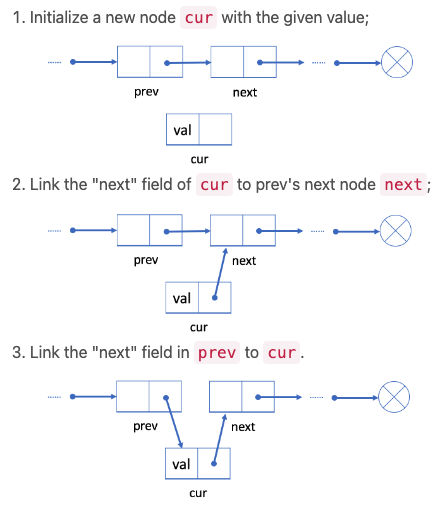
\includegraphics[width=0.6\textwidth]{/insert-into-singly-linked-list.png}
  \caption{Insert into singled linked list}
  \label{fig:insert-into-linked-list}
\end{figure}



\subsection{Delete}


Figure \ref{fig:delete-from-singled-linked-list} shows the operations to delete an existing node \keyword{cur} from the singly linked list.

\begin{figure}[!ht]
  \centering
  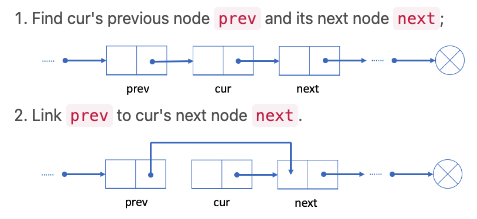
\includegraphics[width=0.6\textwidth]{/delete-from-singled-linked-list.png}
  \caption{Delete from singled linked list}
  \label{fig:delete-from-singled-linked-list}
\end{figure}



\section{Doubly Linked List}
\label{sec:doubly-linked-list}

The doubly linked list works in a similar way but has one more reference field which is known as the ``prev'' field.
With this extra field, you are able to know the previous node of the current node.


\subsection{Add Operation}
\label{sec:add-operation}

If we want to insert a new node \keyword{cur} after an existing node \keyword{prev}, we can divide this process into two steps as shown in Figure \ref{fig:add-to-doubly-linked-list}.
\begin{figure}[!ht]
  \centering
  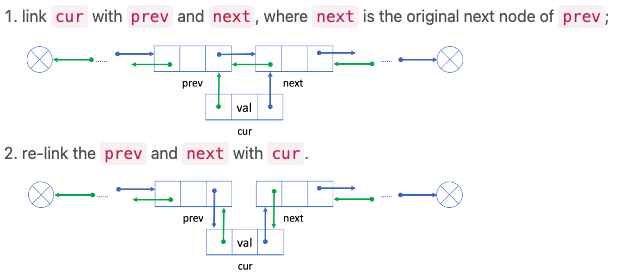
\includegraphics[width=0.8\textwidth]{/add-to-doubly-linked-list.png}
  \caption{Add to linked list}
  \label{fig:add-to-doubly-linked-list}
\end{figure}



\subsection{Delete Operation}
\label{sec:delete-operation}

If we want to delete an existing node \keyword{cur} from the doubly linked list, we can simply link its previous node \keyword{prev} with its next node \keyword{next}.



\section{Comparison}
\label{sec:comparison}



Here we provide a comparison of time complexity between the linked list and the array shown in Figure \ref{fig:array-and-linked-list}.
\begin{figure}[!ht]
  \centering
  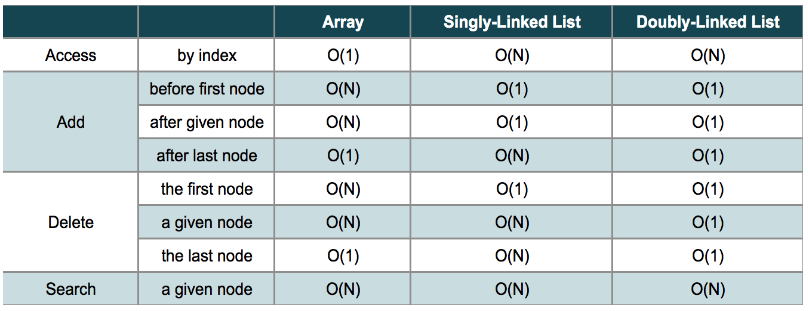
\includegraphics[width=0.8\textwidth]{/array-linked-list-comparison.png}
  \caption{Array and Linked List}
  \label{fig:array-and-linked-list}
\end{figure}


\section{Examples}
\label{sec:examples}


Here are some codes about linked list on \href{https://github.com/mingmingli916/algorithms/tree/main/linked_list}{Github}.



%%% Local Variables:
%%% mode: latex
%%% TeX-master: "algorithms"
%%% End:


\chapter{Binary Tree}
\label{cha:binary-tree}

A \keyword{tree} is a frequently-used data structure to simulate a hierarchical tree structure.
Each node of the tree will have a \keyword{root} value and a list of references to other nodes which are called \keyword{child} nodes.



A \keyword{Binary Tree} is one of the most typical tree structure.
As the name suggests, a binary tree is a tree data structure in which each node has at most two children, which are referred to as the \keyword{left} child and the \keyword{right} child, as shown in Figure \ref{fig:binary-tree}.
\begin{figure}[!ht]
  \centering
  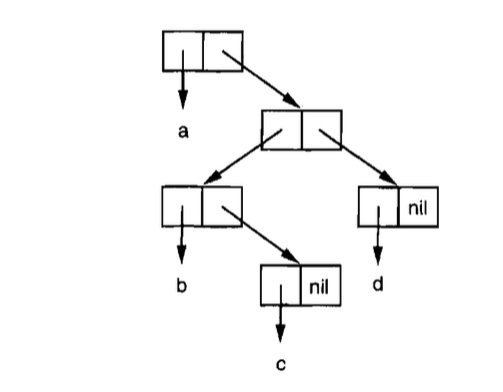
\includegraphics[width=0.6\textwidth]{binary-tree.png}
  \caption{Binary tree}
  \label{fig:binary-tree}
\end{figure}






\section{Traverse a Tree}
\label{sec:traverse-tree}

There are 4 common used traversal:
\begin{itemize}
\item Pre-order Traversal
\item In-order Traversal
\item Post-order Traversal
\item Level-order Traversal
\end{itemize}


The pre-in-post order references the \keyword{root}.

Pre-order traversal is to visit the \keyword{root} first.
Then traverse the left subtree.
Finally, traverse the right subtree.

In-order traversal is to traverse the left subtree first.
Then visit the \keyword{root}.
Finally, traverse the right subtree.

Post-order traversal is to traverse the left subtree first.
Then traverse the right subtree.
Finally, visit the \keyword{root}.

Level-order traversal is to traverse the nodes by level from root to leaves.
In the same level, traverse from left to right.

Take the Figure \ref{fig:binary-tree} for example.
Pre-order traversal generate the sequence: \([8\ 3\ 1\ 6\ 4\ 7\ 10\ 14\ 13]\).
In-order traversal generate the sequence: \([1\ 3\ 4\ 6\ 7\ 8\ 10\ 13\ 14]\).
Post-order traversal generate the sequence: \([1\ 4\ 7\ 6\ 3\ 13\ 14\ 10\ 8]\).
Level-order traversal generate the sequence: \([8\ 3\ 10\ 1\ 6\ 14\ 4\ 7\ 13]\).


\section{Examples}
\label{sec:examples-1}

Here are some codes about binary tree on \href{https://github.com/mingmingli916/algorithms/tree/main/binary_tree}{Github}.

%%% Local Variables:
%%% mode: latex
%%% TeX-master: "algorithms"
%%% End:


\chapter{N-ary Tree}
\label{cha:n-ary-tree}

If a tree is a rooted tree in which each node has no more than \argument{N} children, it is called \keyword{N-ary tree}.


Here is an example of 3-ary tree:
\begin{figure}[H]
  \centering
  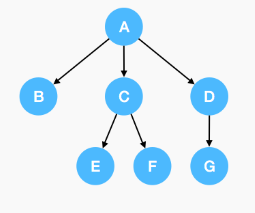
\includegraphics[width=0.5\textwidth]{n-ary-tree}
  \caption{N-ary tree}
  \label{fig:n-ary-tree}
\end{figure}

\keyword{Trie} (Chapter \ref{cha:trie}) is one of the most frequently used N-ary trees.

\section{Travesal}
\label{sec:travesal}


A binary tree can be traversed in preorder, inorder, postorder or level-order.
Among these traversal methods, preorder, postorder and level-order traversal are suitable to be extended to an \keyword{N-ary tree}.


\section{Examples}
\label{sec:examples-5}

Here are some examples on \href{https://github.com/mingmingli916/algorithms/tree/main/n_ary_tree}{Github}.



%%% Local Variables:
%%% mode: latex
%%% TeX-master: "algorithms"
%%% End:


\chapter{Trie}
\label{cha:trie}

A Trie is a special form of a N-ary tree.
Typically, a trie is used to store strings.
Each Trie node represents a string (a prefix).
Each node might have several children nodes while the paths to different children nodes represent different characters.
And the strings the child nodes represent will be the origin string represented by the node itself plus the character on the path.



One important property of Trie is that all the descendants of a node have a common prefix of the string associated with that node.
That's why Trie is also called prefix tree.


\section{How to represent a Trie?}

There are a lot of different representations of a trie node.
Here we provide two of them.

\subsection{Array}

The first solution is to use an array to store children nodes.

For instance, if we store strings which only contains letter a to z, we can declare an array whose size is 26 in each node to store its children nodes.
And for a specific character c, we can use c - 'a' as the index to find the corresponding child node in the array.
Here's the Python code.
\begin{lstlisting}[language=python]
class TrieNode:
    def __init__(self, N=26):
        # you might need some extra values according to different cases
        self.N = N
        self.children = [''] * self.N

# Usesage.
# Initialization
root = TrieNode()
# Return a specific child node with char c
root[ord[c] - ord['a']]
\end{lstlisting}

It is really fast to visit a child node.
It is comparatively easy to visit a specific child since we can easily transfer a character to an index in most cases.
But not all children nodes are needed.
So there might be some waste of space.


\subsection{Hashmap}

The second solution is to use a hashmap to store children nodes.
Here's the Python code.
\begin{lstlisting}
class TrieNode:
    def __init__(self):
        self.children = {}

# Usesage.
# Initialization
root = TrieNode()
# Return a specific child node with char c
root[c]
\end{lstlisting}

It is even easier to visit a specific child directly by the corresponding character.
But it might be a little slower than using an array.
However, it saves some space since we only store the children nodes we need.
It is also more flexible because we are not limited by a fixed length and fixed range.

\section{Insertion in Trie}


Here is the pseudo-code:
\begin{lstlisting}
1. Initialize: cur = root
2. for each char c in target string S:
3.   if cur does not have a child c:
4.     cur.children[c] = new Trie node
5.     cur = cur.children[c]
6. cur is the node which represents the string S  
\end{lstlisting}



\section{Search in Trie}

\subsection{Search prefix}

Here is the pseudo-code:
\begin{lstlisting}
1. Initialize: cur = root
2. for each char c in target string S:
3.   if cur does not have a child c:
4.     search fails
5.   cur = cur.children[c]
6. search successes  
\end{lstlisting}


\subsection{Search word}


You might also want to know how to search for a specific word rather than a prefix.
We can treat this word as a prefix and search in the same way we mentioned above.  


\begin{enumerate}
\item If search fails which means that no words start with the target word, the target word is definitely not in the Trie.
\item If search succeeds, we need to check if the target word is only a prefix of words in Trie or it is exactly a word. 
\end{enumerate}


\section{Examples}
\label{sec:examples-3}

Here are some codes about hash table on \href{https://github.com/mingmingli916/algorithms/tree/main/trie}{Github}


%%% Local Variables:
%%% mode: latex
%%% TeX-master: "algorithms"
%%% End:


\chapter{Queue and Stack}
\label{cha:queue-stack}

\section{Queue}
\label{sec:queue}

Queue is first in first out data structure.
In a FIFO data structure, the first element added to the queue will be processed first.
It is like an array, but the elements can be put into the queue at the end ant put out of the queue at the front.
As show in Figure \ref{fig:queue}.
\begin{figure}[!ht]
  \centering
  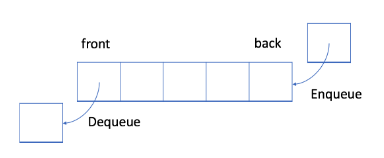
\includegraphics[width=0.8\textwidth]{queue.png}
  \caption{Queue}
  \label{fig:queue}
\end{figure}

There are two operations:
\begin{itemize}
\item enqueue: insert a new element at the end of the queue
\item dequeue: remove the element at the front(head) of the queue
\end{itemize}




\subsection{Queue and BFS}
\label{sec:queue-bfs}

Queue is usually used in BFS (Breadth-first Search).

Here is a simple template (Python):
\lstset{language=Python}
\begin{lstlisting}
  def BFS(root, target) -> int:
    queue = []
    step = 0
    queue.append(root)
    while queue:
        for node in queue:
            if node == target:
                return step
            # Add all node neighbors into the queue
            for neighbor in node.neighbors:
                queue.append(neighbor)
            queue.pop(0)
        step += 1
    # There is no path from root to target.
    return -1

\end{lstlisting}

\section{Stack}
\label{sec:stack}

Stack is last in first out data structure.
In a LIFO structure, the newest element added to the queue will be processed first.
It is like an array, but the elements can be put into the stack and put out of the queue at the end.
As show in Figure \ref{fig:stack}
\begin{figure}[!ht]
  \centering
  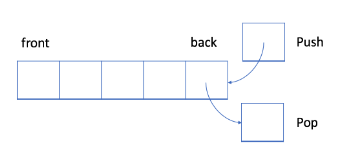
\includegraphics[width=0.8\textwidth]{stack.png}
  \caption{Stack}
  \label{fig:stack}
\end{figure}


There are two operations:
\begin{itemize}
\item push: add a new element at the end(top) of the stack
\item pop: remove the element at the end(top) of the stack
\end{itemize}

\subsection{Stack and DFS}
\label{sec:stack-dfs}

In most cases, we can also use DFS when using BFS. But there is an important difference: the traversal order.
Different from BFS, the nodes you visit earlier might not be the nodes which are closer to the root node.
As a result, the first path you found in DFS might not be the shortest path.

Here is a simple template (Python):
\lstset{language=Python}
\begin{lstlisting}
  def DFS(cur, target, visited: set) -> bool:
    if cur == target:
        return True
    for nei in cur.neighbors:
        if nei not in visited:
            visited.add(nei)
        if DFS(nei, target, visited):
            return True
    return False
\end{lstlisting}


The advantage of the recursion solution is that it is easier to implement.
However, there is a huge disadvantage: if the depth of recursion is too high, you will suffer from stack overflow.
In that case, you might want to use BFS instead or implement DFS using an explicit stack.

\section{Examples}
\label{sec:examples-2}

Here are some example on \href{https://github.com/mingmingli916/algorithms/tree/main/queque_and_stack}{Github}.



  


%%% Local Variables:
%%% mode: latex
%%% TeX-master: "algorithms"
%%% End:


\chapter{Hash Table}

\keyword{Hash Table} is a data structure which organizes data using hash functions in order to support quick insertion and search.

The key idea of Hash Table is to use a hash function to map keys to buckets.
To be more specific,
\begin{itemize}
\item When we insert a new key, the hash function will decide which bucket the key should be assigned and the key will be stored in the corresponding bucket;
\item When we want to search for a key, the hash table will use the \keyword{same} hash function to find the corresponding bucket and search only in the specific bucket.
\end{itemize}

For example in Figure:
\begin{figure}[!ht]
  \centering
  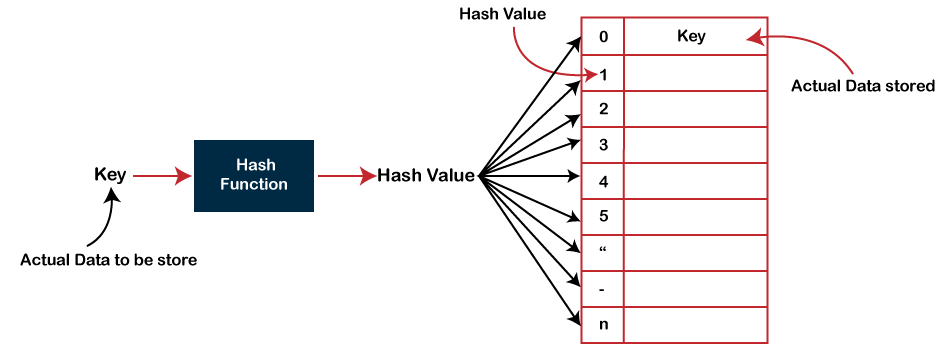
\includegraphics[width=0.7\textwidth{}]{hash-table.png}
  \caption{Hash table}
  \label{fig:hash-table}
\end{figure}


\section{Designing a Hash Table}
\label{sec:designing-hash-table}

There are two essential factors that you should pay attention to when you are going to design a hash table: hash function and collision resolution.

\subsection{Hash Function}
\label{sec:hash-function}

The hash function is the most important component of a hash table which is used to map the key to a specific bucket.
The hash function will depend on \keyword{the range of key values} and \keyword{the number of buckets}.
It is an open problem to design a hash function.
The idea is to try to assign the key to the bucket as \keyword{uniformly} as you can.
Ideally, a perfect hash function will be a one-one mapping between the key and the bucket.
However, in most cases, a hash function is not perfect and it is a tradeoff between the amount of buckets and the capacity of a bucket.


\subsection{Collision Resolution}
\label{sec:collision-resolution}

Ideally, if our hash function is a perfect one-one mapping, we will not need to handle collisions.
Unfortunately, in most cases, collisions are almost inevitable.

A collision resolution algorithm should solve the following questions:
\begin{enumerate}
\item How to organize the values in the same bucket?
\item What if too many values are assigned to the same bucket?
\item How to search for a target value in a specific bucket?
\end{enumerate}

These questions are related to the capacity of the bucket and the number of keys which might be mapped into the same bucket according to our hash function. 
Let's assume that the bucket, which holds the maximum number of keys, has N keys.
Typically, if N is constant and small, we can simply use an array to store keys in the same bucket.
If N is variable or large, we might need to use height-balanced binary search tree instead.

 





\section{Built-in Hash Table}

The typical design of built-in hash table is:
\begin{enumerate}
\item The key can be any \keyword{hashable} type. And a key with belongs to a hashable type will have a \keyword{hashcode}. This code will be used in the mapping function to get the bucket index.
\item Each bucket contains \keyword{an array} to store all the values in the same bucket initially.
\item If there are two many values the same bucket, these values will be maintained in a \keyword{height-balanced binary search tree} instead.
\end{enumerate}

The average time complexity of both insertion and search is still \keyword{O(1)}.
And the time complexity in the worst case is \keyword{O(logN)} for both insertion and search by using height-balanced BST.



\section{Designing a Key Example}

Sometimes you have to think it over to design a suitable key when using a hash table.


For example:


Given an array of strings, group anagrams\footnote{An Anagram is a word or phrase formed by rearranging the letters of a different word or phrase, typically using all the original letters exactly once.} together.  




As we know, a hash map can perform really well in grouping information by key.
But we cannot use the original string as key directly.
We have to design a proper key to present the type of anagrams.
For instance,  "eat" and "ate" should be in the same group.
While "eat" and "act" should not be grouped together.


When you design a key, you need to guarantee that:
\begin{enumerate}
\item All values belong to the same group will be mapped in the same group.\label{item:1}
\item Values which needed to be separated into different groups will not be mapped into the same group.\label{item:2}
\end{enumerate}


\begin{lstlisting}[language=python]
class Solution:
    def groupAnagrams(self, strs: List[str]) -> List[List[str]]:
        d = collections.defaultdict(list)
        for s in strs:
            hashkey = self.hash(s)
            d[hashkey].append(s)
        return list(d.values())

    def hash(self, s: str) -> str:
        return ''.join(sorted(s))        
\end{lstlisting}

This process is similar to design a hash function, but here is an essential difference.
A hash function satisfies rule \ref{item:1} but might not satisfy rule \ref{item:2}.
But your mapping function should satisfy both of them.






\subsection{Summary}

Here are some takeaways about how to design the key for you:
\begin{enumerate}
\item When the order of each element in the string/array doesn't matter, you can use the \keyword{sorted string/array} as the key.
\item If you only care about the offset of each value, usually the offset from the first value, you can use the \keyword{offset} as the key.
\item In a tree, you might want to directly use the \keyword{TreeNode} as key sometimes. But in most cases, the \keyword{serialization of the subtree} might be a better idea.
\item In a matrix, you might want to use \keyword{the row index} or \keyword{the column index} as key.
\item In a Sudoku, you can combine the row index and the column index to identify which \keyword{block} this element blongs to.
\item Sometimes, in a matrix, you might want to aggregate the values in the same \keyword{diagonal line}. $(i,j) \rightarrow i+j$, $(i,j) \rightarrow i-j$
\end{enumerate}



\section{Conclusion}

A typical thinking process to solve problems by hash table is show in Figure \ref{fig:how-to-apply-hash-table}:
\begin{figure}[!ht]
  \centering
  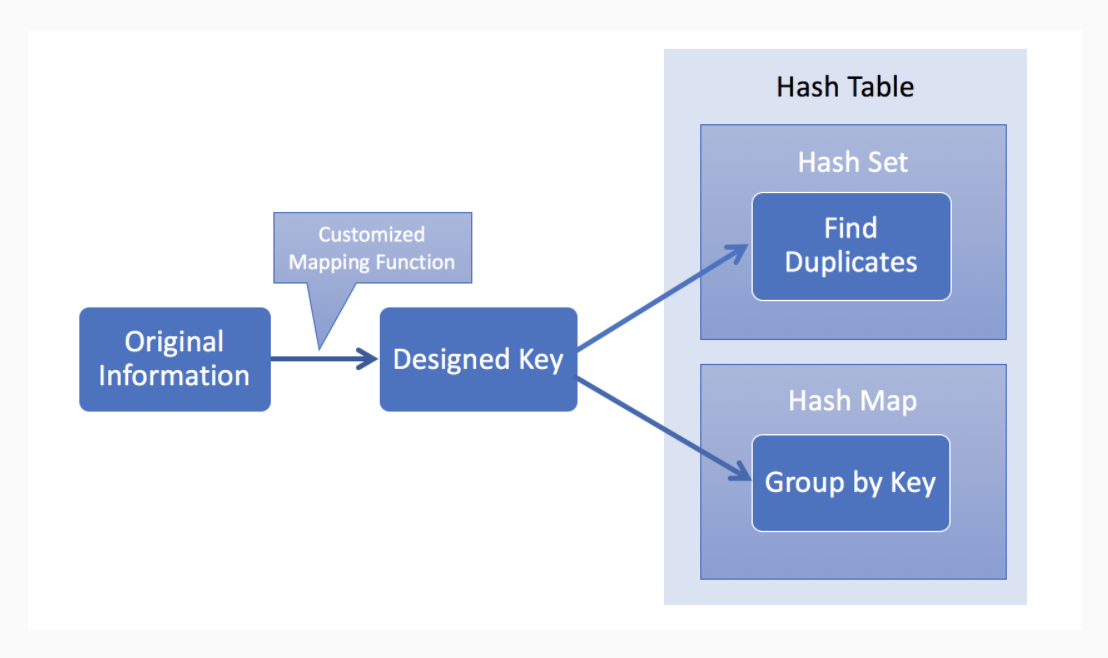
\includegraphics[width=\textwidth]{how-to-apply-hash-table}
  \caption{Thinking process by hash table}
  \label{fig:how-to-apply-hash-table}
\end{figure}



What's more, we will meet more complicated problems sometimes. We might need to:

\begin{itemize}
\item use several hash tables together
\item combine the hash table with other data structure
\item combine the hash table with other algorithms
\item ...
\end{itemize}

%%% Local Variables:
%%% mode: latex
%%% TeX-master: "algorithms"
%%% End:

\section{Examples}
\label{sec:examples-6}

Here are some examples on \href{https://github.com/mingmingli916/algorithms/tree/main/hash_table}{Github}

\part{Algorithm}
\label{part:algorithm}


\chapter{Binary Search}
\label{cha:binary-search}

\keyword{Binary Search} is one of the most fundamental and useful algorithms in Computer Science.
It describes the process of searching for a specific value in an \keyword{ordered} collection.


\section{General Idea}
\label{sec:general-idea}

\begin{figure}[H]
  \centering
  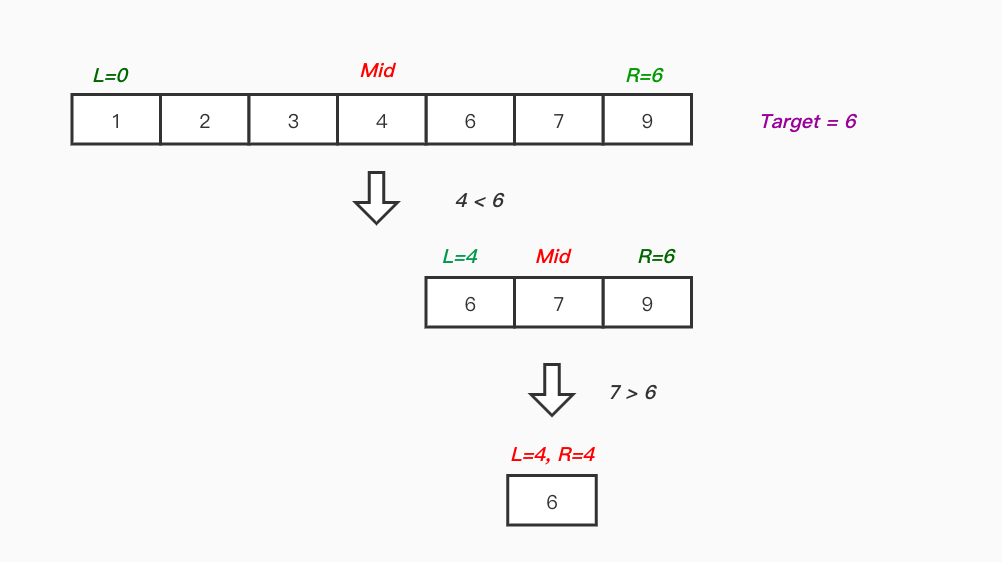
\includegraphics[width=0.8\textwidth]{binary-search}
  \caption{Binary Search}
  \label{fig:binary-search}
\end{figure}

The general process is as follows (if the collection is increase sorted):
\begin{enumerate}
\item Compute the \argument{mid} index.
\item If the value at \argument{mid} is the \argument{target}, search ends.
\item If the \argument{target} is great than the value at \argument{mid}, search the right part of the \argument{mid} else the left.
\item Repeat the previous process till the \argument{target} is found or search end (no more elements to search for).
\end{enumerate}

\section{Templates}
\label{sec:templates}

\subsection{Template 1}
\label{sec:template-1}

\begin{lstlisting}[language=python]
def binarySearch(nums, target):
    """
    :type nums: List[int]
    :type target: int
    :rtype: int
    """
    if len(nums) == 0:
        return -1

    left, right = 0, len(nums) - 1
    while left <= right:
        mid = (left + right) // 2
        if nums[mid] == target:
            return mid
        elif nums[mid] < target:
            left = mid + 1
        else:
            right = mid - 1

    # End Condition: left > right
    return -1
\end{lstlisting}

Template 1 is the most basic and elementary form of Binary Search.
It is used to search for an element or condition which can be determined by accessing \keyword{a single index} in the array.



\subsection{Template 2}
\label{sec:template-2}

\begin{lstlisting}[language=python]
def binarySearch(nums, target):
    """
    :type nums: List[int]
    :type target: int
    :rtype: int
    """
    if len(nums) == 0:
        return -1

    left, right = 0, len(nums)
    while left < right:
        mid = (left + right) // 2
        if nums[mid] == target:
            return mid
        elif nums[mid] < target:
            left = mid + 1
        else:
            right = mid

    # Post-processing:
    # End Condition: left == right
    if left != len(nums) and nums[left] == target:
        return left
    return -1

\end{lstlisting}

Template 2 is an advanced form of Binary Search.
It is used to search for an element or condition which requires accessing \keyword{the current index and its immediate right neighbor's index} in the array.

\subsection{Template 3}
\label{sec:template-3}

\begin{lstlisting}
def binarySearch(nums, target):
    """
    :type nums: List[int]
    :type target: int
    :rtype: int
    """
    if len(nums) == 0:
        return -1

    left, right = 0, len(nums) - 1
    while left + 1 < right:
        mid = (left + right) // 2
        if nums[mid] == target:
            return mid
        elif nums[mid] < target:
            left = mid
        else:
            right = mid

    # Post-processing:
    # End Condition: left + 1 == right
    if nums[left] == target: return left
    if nums[right] == target: return right
    return -1
\end{lstlisting}

Template 3 is another form of Binary Search.
It is used to search for an element or condition which requires accessing \keyword{the current index and its immediate left and right neighbor's index} in the array.

\section{Time and Space Complexity}
\label{sec:time-space-compl}

\subsection{Time Complexity}
\label{sec:time-complexity}


Logarithmic Time: \(O(\log n)\)

Because Binary Search operates by applying a condition to the value in the middle of our search space and thus cutting the search space in half, in the worse case, we will have to make \(O(\log n)\) comparisons, where \(n\) is the number of elements in our collection.

 \subsection{Space Complexity}
\label{sec:space-complexity}

Constant Space: \(O(1)\)

Although Binary Search does require keeping track of 3 indices, the iterative solution does not typically require any other additional space and can be applied directly to the collection itself, therefore warrants \(O(1)\) or constant space.


\section{Examples}
\label{sec:examples-4}

Here are some examples on \href{https://github.com/mingmingli916/algorithms/tree/main/binary_search}{Github}.
%%% Local Variables:
%%% mode: latex
%%% TeX-master: "algorithms"
%%% End:


\chapter{Sorting}
\label{cha:sorting}

In computer science, we have formal definitions of sorting with respect to ordering relations.

An ordering relation has two key properties:
\begin{enumerate}
\item Given two elements \(a\) and \(b\), exactly one of the following must be true: \(a < b, a = b\) or \(a > b\) (law of trichotomy)
\item If \(a < b\) and \(b < c\) then \(a < c\) (law of transitivity)
\end{enumerate}



A \keyword{sort} is formally defined as a rearrangement of a sequence of elements that puts all elements into a non-decreasing order based on the ordering relation.


An important concept in sorting is \keyword{inversions}.
An inversion in a sequence is defined as a pair of elements that are out of order with respect to the ordering relation.
For example, \(1, 2, 4, 6, 5, 3\).
The inversions are \((4,3), (6,5), (6,3), (5,3)\).
There are 4 inversions in the previous list.


The next important concept in sorting is the \keyword{stability} of sorting algorithms.
The key feature of a stable sorting algorithm is that it will preserve the order of equal elements.
For example, [“hello”, “world”, “we”, “are”, “learning, “sorting”].
We define an ordering relation based on the length of the string.
There are two valid sorts for this sequence:
\begin{enumerate}
\item “we”, “are”, “hello”, “world”, “sorting”, “learning”
\item “we”, “are”, “world”, “hello”, “sorting”, “learning”
\end{enumerate}

We consider (1) to be a stable sort since the equal elements “hello” and “world” are kept in the same relative order as the original sequence.



\section{Comparison Based Sort}
\label{sec:comp-based-sort}

Comparison based sorts are sorting algorithms that require a direct method of comparison defined by the ordering relation.
In a sense, they are the most natural sorting algorithms since, intuitively, when we think about sorting elements, we instinctively think about comparing elements to each other.

\subsection{Selection Sort}
\label{sec:selection-sort}

Suppose we had a collection of elements where every element is an integer.
Selection sort will build up the sorted list by repeatedly \keyword{selecting} the minimum element in that list and moving it to the front of the list through a swap.
It will proceed to swap elements appropriately until the entire list is sorted.

\begin{figure}[H]
  \centering
  \myfigure[0.5]{selection-sort}
  \caption{Selection sort}
\end{figure}

It's time complexity is \(O(n^{2})\) and space complexity is \(O(1)\).
It is not a stable sorting algorithm.

\begin{lstlisting}
class Solution:
    def selection_sort(self, lst: List[int]) -> None:
        """
        Mutates lst so that it is sorted via selecting the minimum element and swapping it with the corresponding index.
        """
        for i in range(len(lst)):
            min_index = i
            for j in range(i + 1, len(lst)):
                # Update minimum index
                if lst[j] < lst[min_index]:
                    min_index = j

            # Swap current index with minimum element in rest of list
            lst[min_index], lst[i] = lst[i], lst[min_index]
\end{lstlisting}



\subsection{Bubble Sort}
\label{sec:bubble-sort}

Suppose we have a collection of integers that we want to sort in ascending order.
Bubble sort proceeds to consider two adjacent elements at a time.
If these two adjacent elements are out of order (in this case, the left element is strictly greater than the right element), bubble sort will swap them.
It then proceeds to the next pair of adjacent elements.
In the first pass of bubble sort, it will process every set of adjacent elements in the collection once, making swaps as necessary.
The core idea of bubble sort is it will repeat this process until no more swaps are made in a single pass, which means the list is sorted.



Bubble sort runtime of \(O(n^{2})\).
The space complexity of bubble sort is \(O(1)\).
Bubble sort is also a stable sorting algorithm since equal elements will never have swapped places, so their relative ordering will be preserved.


Overall, bubble sort is fairly simple to implement, and it’s stable, but outside of that, this algorithm does not have many desirable features.
It’s fairly slow for most inputs and, as a result, it is rarely used in practice.



\begin{lstlisting}[language=python]
class Solution:
    def bubble_sort(self, lst: List[int]) -> None:
        """
        Mutates lst so that it is sorted via swapping adjacent elements until
        the entire lst is sorted.
        """
        has_swapped = True
        # if no swap occurred, lst is sorted
        while has_swapped:
            has_swapped = False
            for i in range(len(lst) - 1):
                if lst[i] > lst[i + 1]:
                    # Swap adjacent elements
                    lst[i], lst[i + 1] = lst[i + 1], lst[i]
                    has_swapped = True          
\end{lstlisting}

\subsection{Selection Sort}
\label{sec:selection-sort-1}

Given a collection of integers, you can sort the list by proceeding from the start of the list, and every time you encounter an element that is out of order, you can continuously swap places with previous elements until it is inserted in its correct relative location based on what you’ve processed thus far.

The time complexity is \(O(n^{2})\) and space complexity is \(O(1)\).
It is a stable sort.


There are cases where insertion sort may actually be the best sort.
\begin{itemize}
\item On almost sorted arrays where the number of inversions is relatively small compared to the size of the array, insertion sort will be quite fast since the number of swaps required will be low on almost sorted arrays.
\item Insertion sort can also be the best choice on small arrays.
\end{itemize}


\begin{lstlisting}
class Solution:
    def insertion_sort(self, lst: List[int]) -> None:
        """
        Mutates elements in lst by inserting out of place elements into appropriate
        index repeatedly until lst is sorted
        """
        for i in range(1, len(lst)):
            current_index = i

            while current_index > 0 and lst[current_index - 1] > lst[current_index]:
                # Swap elements that are out of order
                lst[current_index], lst[current_index - 1] = lst[current_index - 1], lst[current_index]
                current_index -= 1
\end{lstlisting}


%%% Local Variables:
%%% mode: latex
%%% TeX-master: "algorithms"
%%% End:


% Pages are numbered with Arabic numbers.
% Chapters generate a table of contents entry but don't get a number.
\backmatter{}
\cleardoublepage{}
\phantomsection{}
\nocite{*}
\bibliographystyle{plain}       % % plain, unsrt, alpha, abbrv
\bibliography{tex}

\cleardoublepage{}
% just setting an anchor like \hypertarget{}{}
% fix the problem that anchor point to the previous section
\phantomsection{}                 
\printindex{}
\end{document}

%%% Local Variables:
%%% mode: latex
%%% TeX-master: t
%%% End:


